\documentclass{article}
\usepackage{amsfonts, amsthm, amsmath, amssymb, mathtools, ulem, mathrsfs, physics, esint, siunitx, tikz-cd}
\usepackage{pdfpages, fullpage, color, microtype, cancel, textcomp, markdown, hyperref, graphicx}
\usepackage{enumitem}
\usepackage{algorithm}
\usepackage{algpseudocode}
\graphicspath{{./images/}}
\usepackage[english]{babel}
\usepackage[autostyle, english=american]{csquotes}
\MakeOuterQuote{"}
\usepackage{xparse}
\usepackage{tikz}

\usepackage{calligra}
\DeclareMathAlphabet{\mathcalligra}{T1}{calligra}{m}{n}
\DeclareFontShape{T1}{calligra}{m}{n}{<->s*[2.2]callig15}{}
\newcommand{\script}[1]{\ensuremath{\mathcalligra{#1}}}
\newcommand{\scr}{\script r}

% fonts
\def\mbb#1{\mathbb{#1}}
\def\mfk#1{\mathfrak{#1}}
\def\mbf#1{\mathbf{#1}}
\def\tbf#1{\textbf{#1}}

% common bold letters
\def\bP{\mbb{P}}
\def\bC{\mbb{C}}
\def\bH{\mbb{H}}
\def\bI{\mbb{I}}
\def\bR{\mbb{R}}
\def\bQ{\mbb{Q}}
\def\bZ{\mbb{Z}}
\def\bN{\mbb{N}}

% brackets
\newcommand{\br}[1]{\left(#1\right)}
\newcommand{\sbr}[1]{\left[#1\right]}
\newcommand{\brc}[1]{\left\{#1\right\}}
\newcommand{\lbr}[1]{\left\langle#1\right\rangle}

% vectors
\renewcommand{\i}{\hat{\imath}}
\renewcommand{\j}{\hat{\jmath}}
\renewcommand{\k}{\hat{k}}
\newcommand{\proj}[2]{\text{proj}_{#2}\br{#1}}
\newcommand{\m}[2][b]{\begin{#1matrix}#2\end{#1matrix}}
\newcommand{\arr}[3][\sbr]{#1{\begin{array}{#2}#3\end{array}}}

% misc
\NewDocumentCommand{\seq}{O{n} O{1} O{\infty} m}{\br{#4}_{{#1}={#2}}^{#3}}
\NewDocumentCommand{\app}{O{x} O{\infty}}{\xrightarrow{#1\to#2}}
\newcommand{\sm}{\setminus}
\newcommand{\sse}{\subseteq}
\renewcommand{\ss}{\subset}
\newcommand{\vn}{\varnothing}
\newcommand{\lc}{\epsilon_{ijk}}
\newcommand{\ep}{\epsilon}
\newcommand{\vp}{\varphi}
\renewcommand{\th}{\theta}
\newcommand{\cjg}[1]{\overline{#1}}
\newcommand{\inv}{^{-1}}
\DeclareMathOperator{\im}{im}
\DeclareMathOperator{\id}{id}
\newcommand{\ans}{\tbf{Ans. }}
\newcommand{\pf}{\tbf{Pf. }}
\newcommand{\imp}{\implies}
\newcommand{\impleft}{\reflectbox{$\implies$}}
\newcommand{\ck}{\frac1{4\pi\ep_0}}
\newcommand{\ckb}{4\pi\ep_0}
\newcommand{\sto}{\longrightarrow}
\DeclareMathOperator{\cl}{cl}
\DeclareMathOperator{\intt}{int}
\DeclareMathOperator{\bd}{bd}
\DeclareMathOperator{\Span}{span}
\newcommand{\floor}[1]{\left\lfloor#1\right\rfloor}
\newcommand{\ceil}[1]{\left\lceil#1\right\rceil}
\newcommand{\fxn}[5]{#1:\begin{array}{rcl}#2&\longrightarrow & #3\\[-0.5mm]#4&\longmapsto &#5\end{array}}
\newcommand{\sep}[1][.5cm]{\vspace{#1}}
\DeclareMathOperator{\card}{card}
\renewcommand{\ip}[2]{\lbr{#1,#2}}
\renewcommand{\bar}{\overline}
\DeclareMathOperator{\cis}{cis}
\DeclareMathOperator{\Arg}{Arg}
\newcommand{\ptl}{\partial}

% title
\title{Scientific Computing HW 13}
\author{Ryan Chen}
%\date{\today}
\setlength{\parindent}{0pt}


\begin{document}
	
\maketitle



\section*{Problem 1.}

\begin{enumerate}[label=(\alph*)]
	
\item Using $f(u)=au$,
$$u_j^* = u_j^n - \frac{ak}{h}(u_{j+1}^n - u_j^n)$$
In turn,
\begin{align*}
	u_j^{n+1} &= \frac12\sbr{u_j^n + u_j^n - \frac{ak}{h}(u_{j+1}^n - u_j^n)} - \frac{ak}{2h}\sbr{u_j^n - \frac{ak}{h}(u_{j+1} - u_j^n) - u_{j-1}^n + \frac{ak}{h}(u_j^n - u_{j-1}^n)}\\
	&= u_j^n - \frac{ak}{2h}(u_{j+1}^n - u_j^n + u_j^n - u_{j-1}^n) + \frac{a^2k^2}{2h^2}(u_{j+1}^n - u_j^n - u_j^n + u_{j-1}^n)\\
	&= u_j^n - \frac{ak}{2h}(u_{j+1}^n - u_{j-1}^n) + \frac{a^2k^2}{2h^2}(u_{j+1}^n - 2u_j^n + u_{j-1}^n)
\end{align*}
Which coincides with Lax--Wendroff.
 
\end{enumerate}



\section*{Problem 2.}

\pf Recall $F(u_L,u_R)=f(u^*(u_L,u_R))$. From the fact $f''>0$, $f'$ is increasing. Suppose $u_L\le u_R$. In case 1, from $f'(u_L)\ge0$ we have $f'\ge0$ hence $f$ is increasing, so $F(u_L,u_R)=\min_{u_L\le u\le u_R}f(u)=f(u_L)$. In case 2, from $f'(u_R)\le0$, we have $f'\le0$ hence $f$ is decreasing, so $F(u_L,u_R)=\min_{u_L\le u\le u_R}f(u)=f(u_R)$. In case 3, we have $f$ is increasing, so $(f(u_L)-f(u_R))/(u_L-u_R)>0$ hence $F(u_L,u_R)=f(u_L)$. Similar arguments can be made for when we suppose $u_L>u_R$.



\section*{Problem 3.}

Code: \url{https://github.com/RokettoJanpu/Scientific-Computing-2/blob/main/hw13q3.ipynb}

Lax--Friedrichs:
\begin{center}
	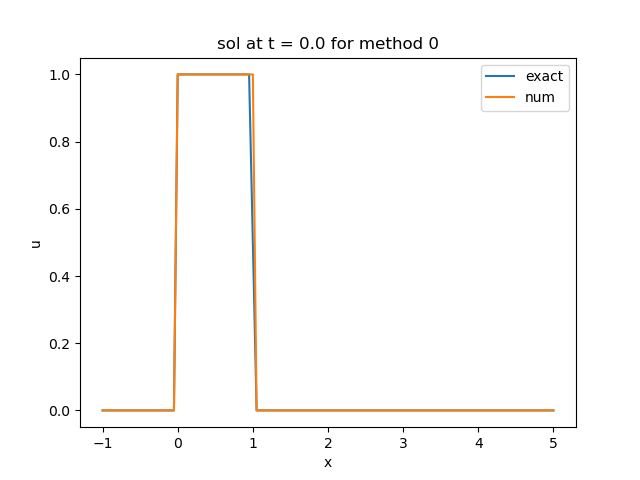
\includegraphics[scale=.23]{hw13 sol t = 0 method 0}
	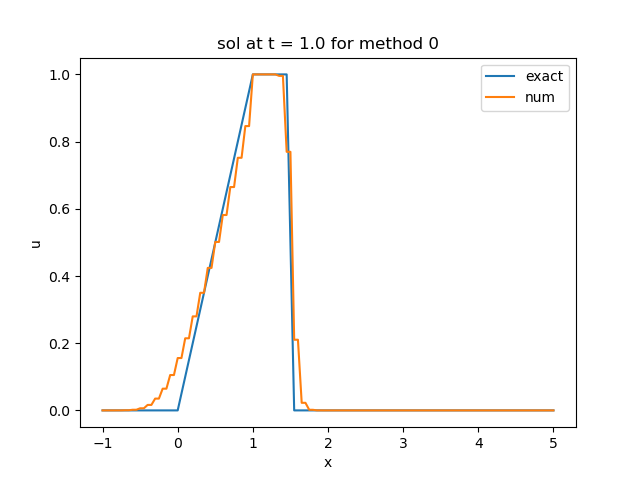
\includegraphics[scale=.23]{hw13 sol t = 1 method 0}
	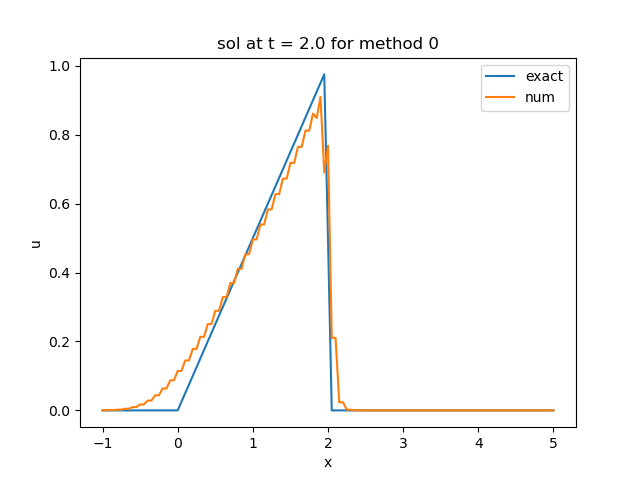
\includegraphics[scale=.23]{hw13 sol t = 2 method 0}
	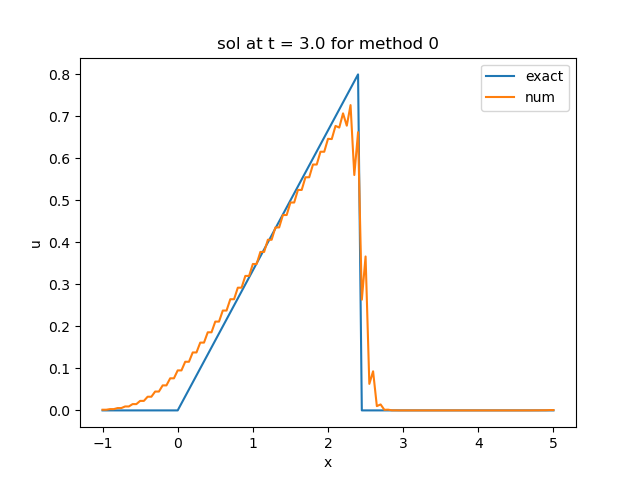
\includegraphics[scale=.23]{hw13 sol t = 3 method 0}
	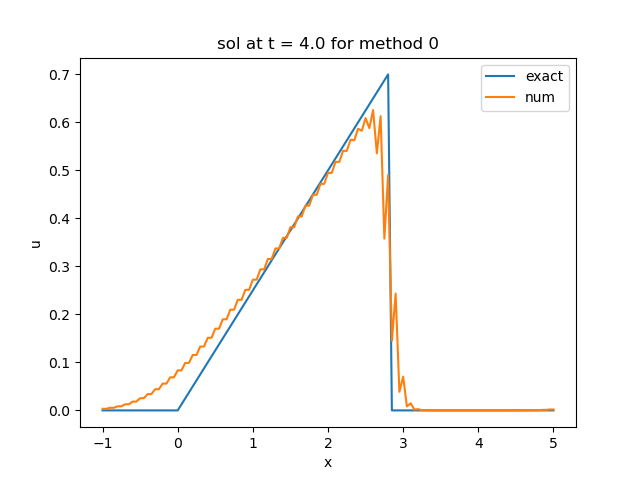
\includegraphics[scale=.3]{hw13 sol t = 4 method 0}
	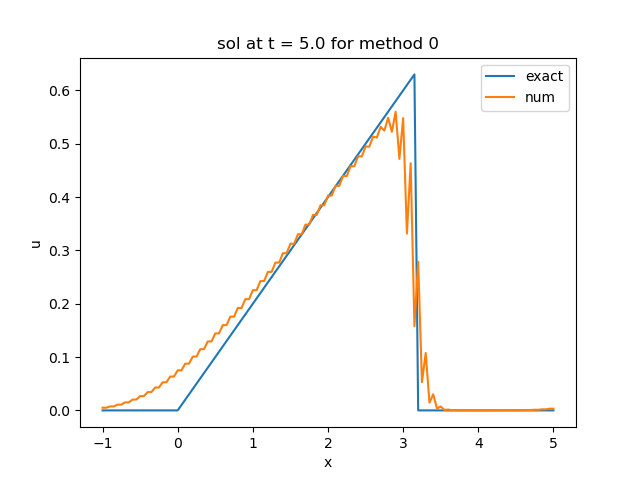
\includegraphics[scale=.3]{hw13 sol t = 5 method 0}
	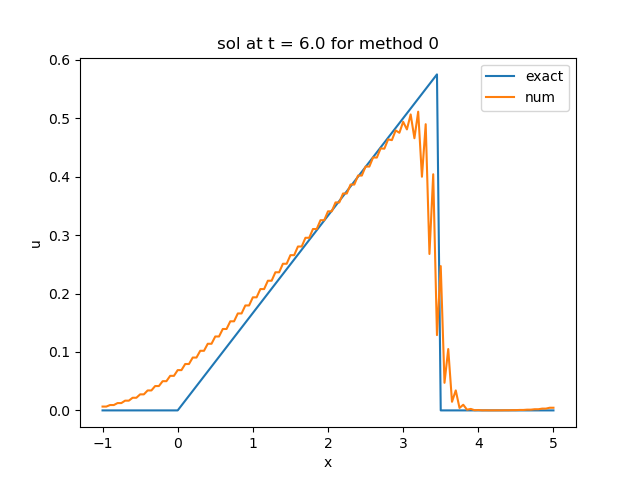
\includegraphics[scale=.3]{hw13 sol t = 6 method 0}
\end{center}
Richtmyer:
\begin{center}
	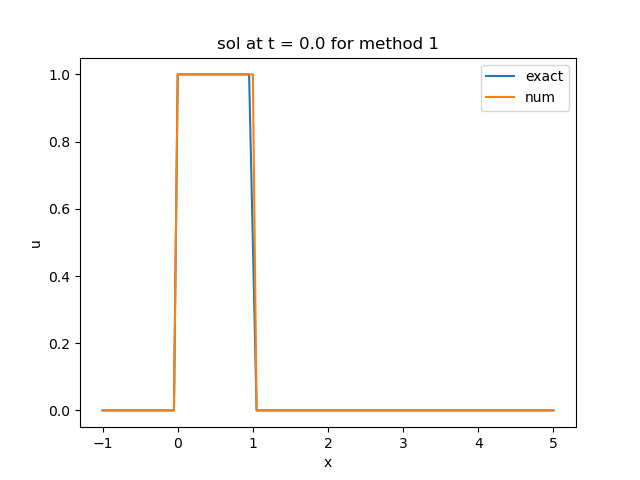
\includegraphics[scale=.23]{hw13 sol t = 0 method 1}
	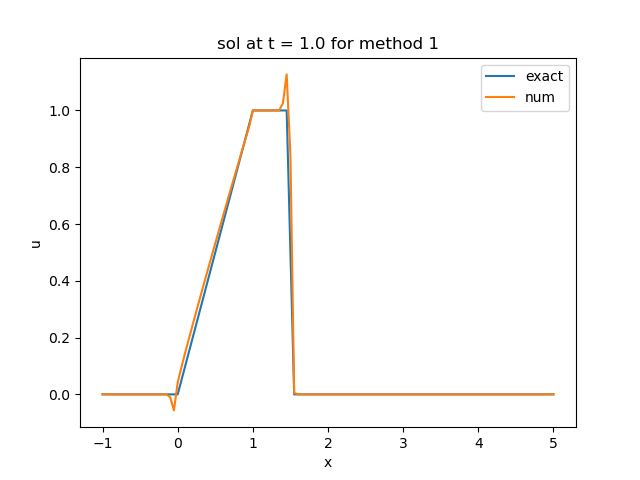
\includegraphics[scale=.23]{hw13 sol t = 1 method 1}
	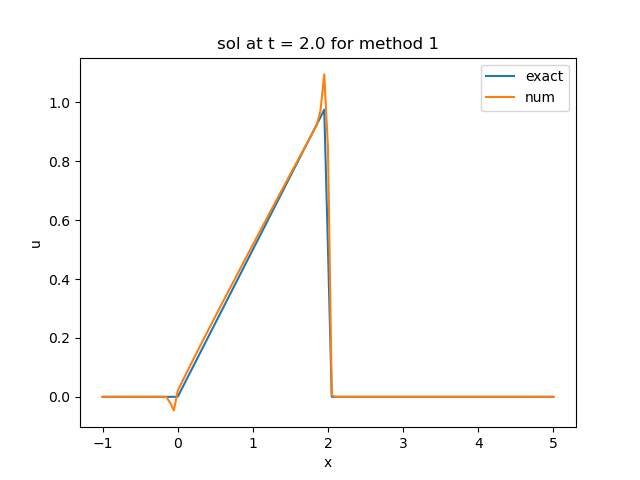
\includegraphics[scale=.23]{hw13 sol t = 2 method 1}
	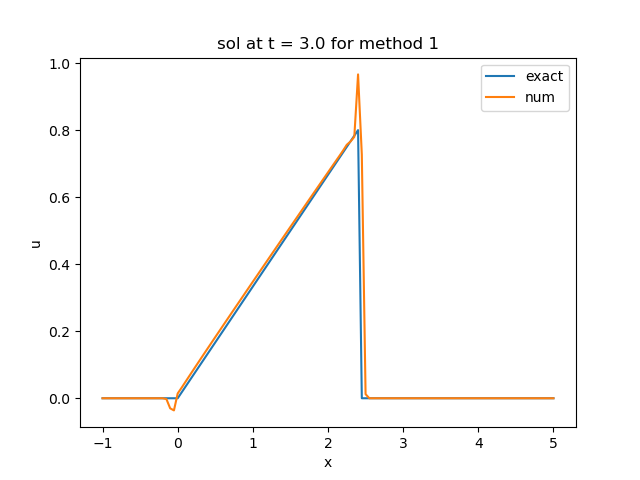
\includegraphics[scale=.23]{hw13 sol t = 3 method 1}
	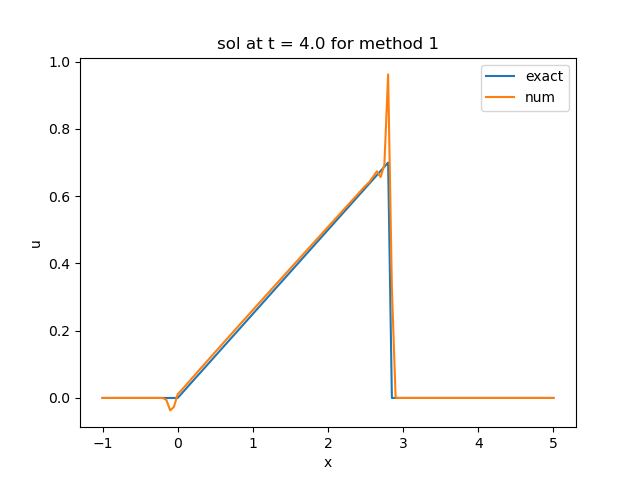
\includegraphics[scale=.3]{hw13 sol t = 4 method 1}
	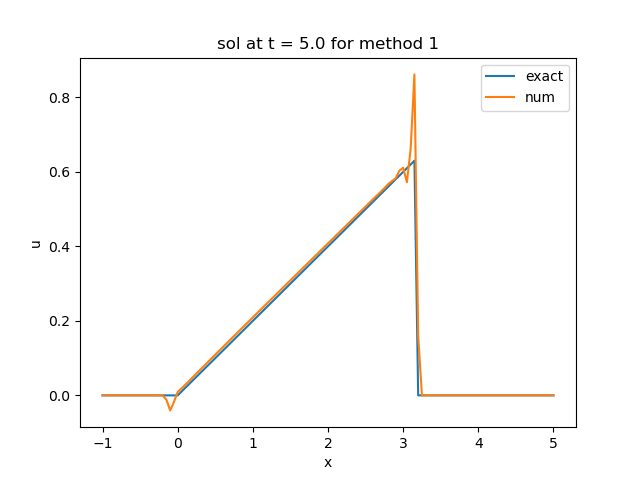
\includegraphics[scale=.3]{hw13 sol t = 5 method 1}
	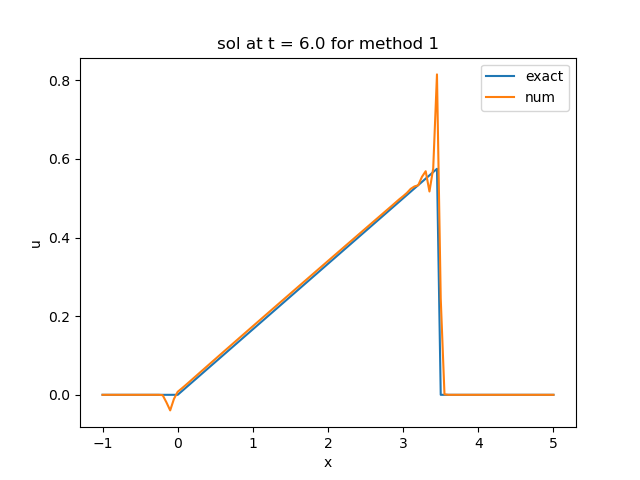
\includegraphics[scale=.3]{hw13 sol t = 6 method 1}
\end{center}
MacCormack:
\begin{center}
	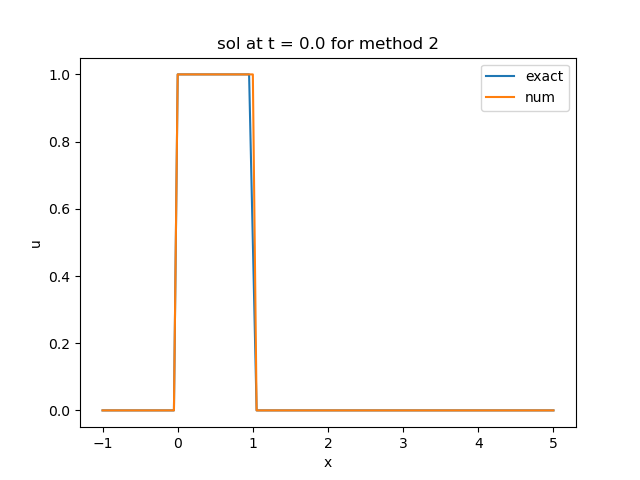
\includegraphics[scale=.23]{hw13 sol t = 0 method 2}
	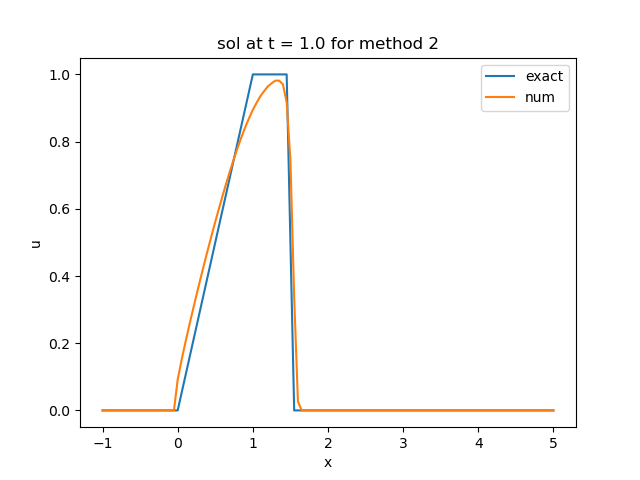
\includegraphics[scale=.23]{hw13 sol t = 1 method 2}
	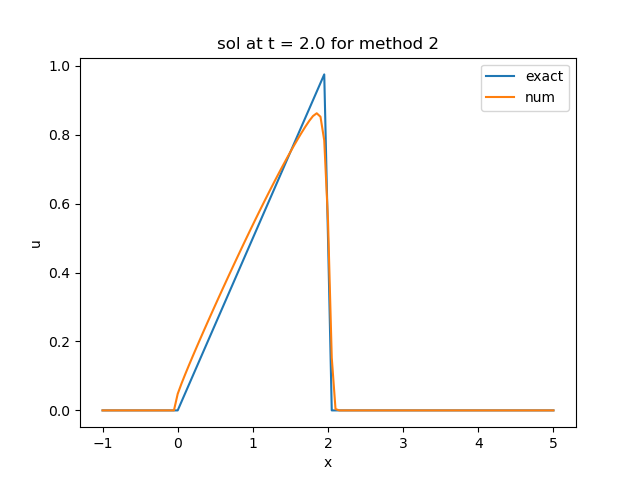
\includegraphics[scale=.23]{hw13 sol t = 2 method 2}
	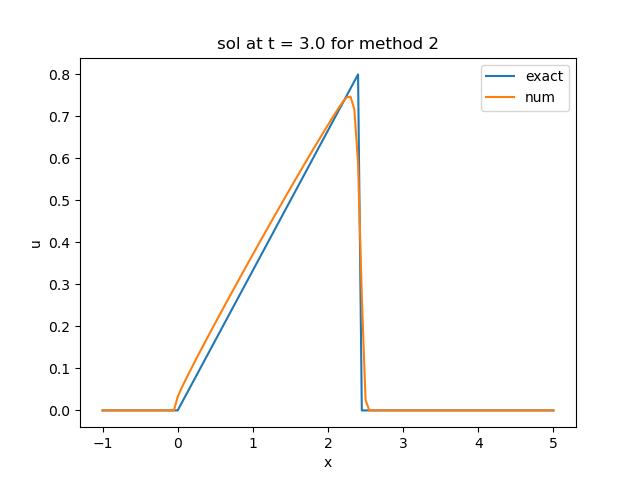
\includegraphics[scale=.23]{hw13 sol t = 3 method 2}
	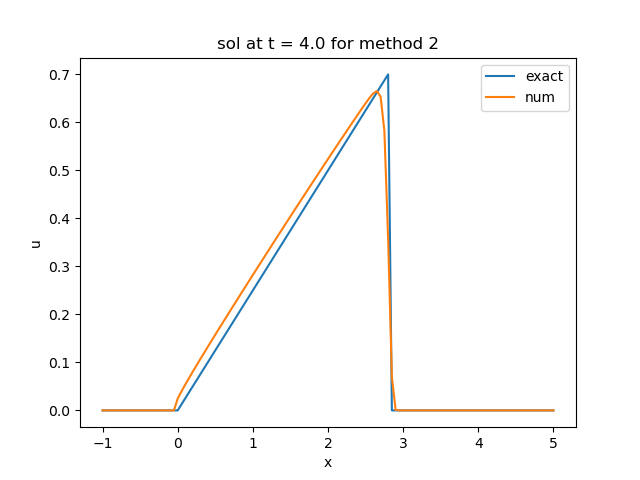
\includegraphics[scale=.3]{hw13 sol t = 4 method 2}
	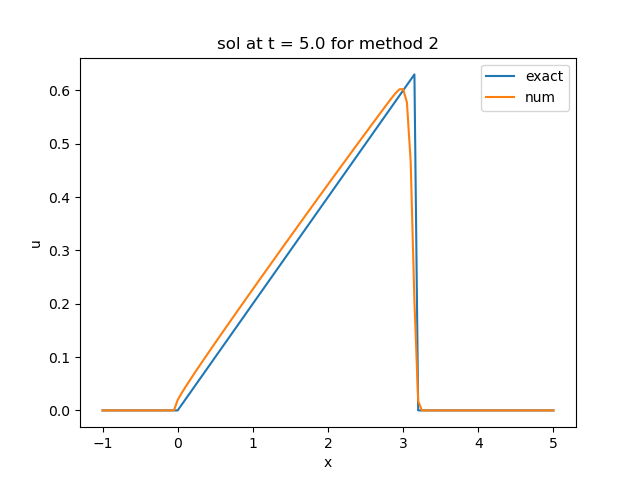
\includegraphics[scale=.3]{hw13 sol t = 5 method 2}
	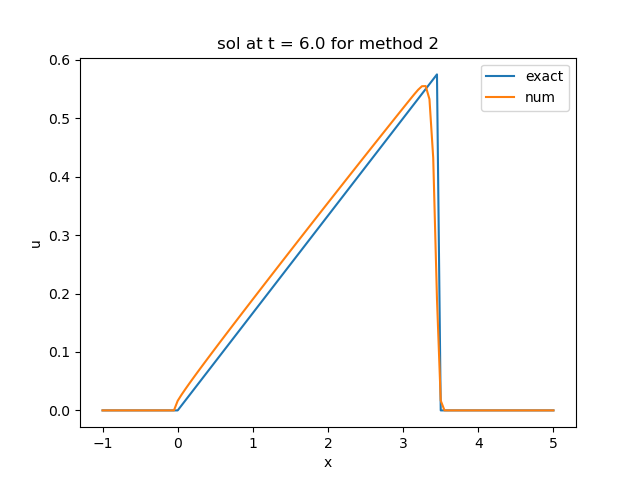
\includegraphics[scale=.3]{hw13 sol t = 6 method 2}
\end{center}

\section*{Problem 4.}
Write the PDE as
$$u_t = \underbrace{-u_{xxxx} - u_{xx}}_{=:Lu} \underbrace{-\frac12(u^2)_x}_{=:N(u)}$$
First solving $u_t=Lu$, write
$$u(x,t) = \sum_{k=-\infty}^{\infty} u_k(t)e^{ikx/16}$$
so that
$$u_t = \sum_{k=-\infty}^{\infty} u_k'(t)e^{ikx/16},
\quad u_{xx} = \sum_{k=-\infty}^{\infty} u_k(t)\br{-\br{\frac{k}{16}}^2}e^{ikx/16},
\quad u_{xxxx} = \sum_{k=-\infty}^{\infty} u_k(t)\br{\frac{k}{16}}^4e^{ikx/16}$$
Plugging in these derivatives and using the fact that the basis functions $e^{ikx/16}$ are linearly independent,
$$u_k'(t) = \sbr{\br{\frac{k}{16}}^2 - \br{\frac{k}{16}}^4}u_k(t)
\imp u_k(t) = u_k(0)e^{[(k/16)^2 - (k/16)^4]t}$$
giving the solution
$$u(x,t) = \sum_{k=-\infty}^{\infty} u_k(0)e^{ikx/16}e^{[(k/16)^2 - (k/16)^4]t},
\quad u_k(0) = \frac{1}{32\pi}\int_0^{32\pi} u(x,0)e^{-ikx/16}dx$$

Define the solution operator $e^{tL}$ by specifying its action on the basis functions $e^{ikx/16}$.
$$e^{tL}(e^{ikx/16}) := e^{ikx/16}e^{[(k/16)^2 - (k/16)^4]t}$$
We check that we can rewrite the solution as
$$u(x,t) = \sum_{k=-\infty}^{\infty} u_k(0)e^{tL}(e^{ikx/16})
= e^{tL}\sum_{k=-\infty}^{\infty} u_k(0)e^{ikx/16}
= e^{tL}u(x,0)$$
Let $v$ satisfy $u=e^{tL}v$. Plugging into the equation $u_t=Lu+N(u)$, we obtain an equation for $v$.
$$Le^{tL}v + e^{tL}v_t = Le^{tL}v + N(e^{tL}v)
\imp e^{tL}v_t = N(e^{tL}v)
\imp v_t = e^{-tL}N(e^{tL}v)$$

The file KdVrkm.m was modified to solve this PDE:

\url{https://github.com/RokettoJanpu/Scientific-Computing-2/blob/main/KdVrkm.m}
\begin{center}
	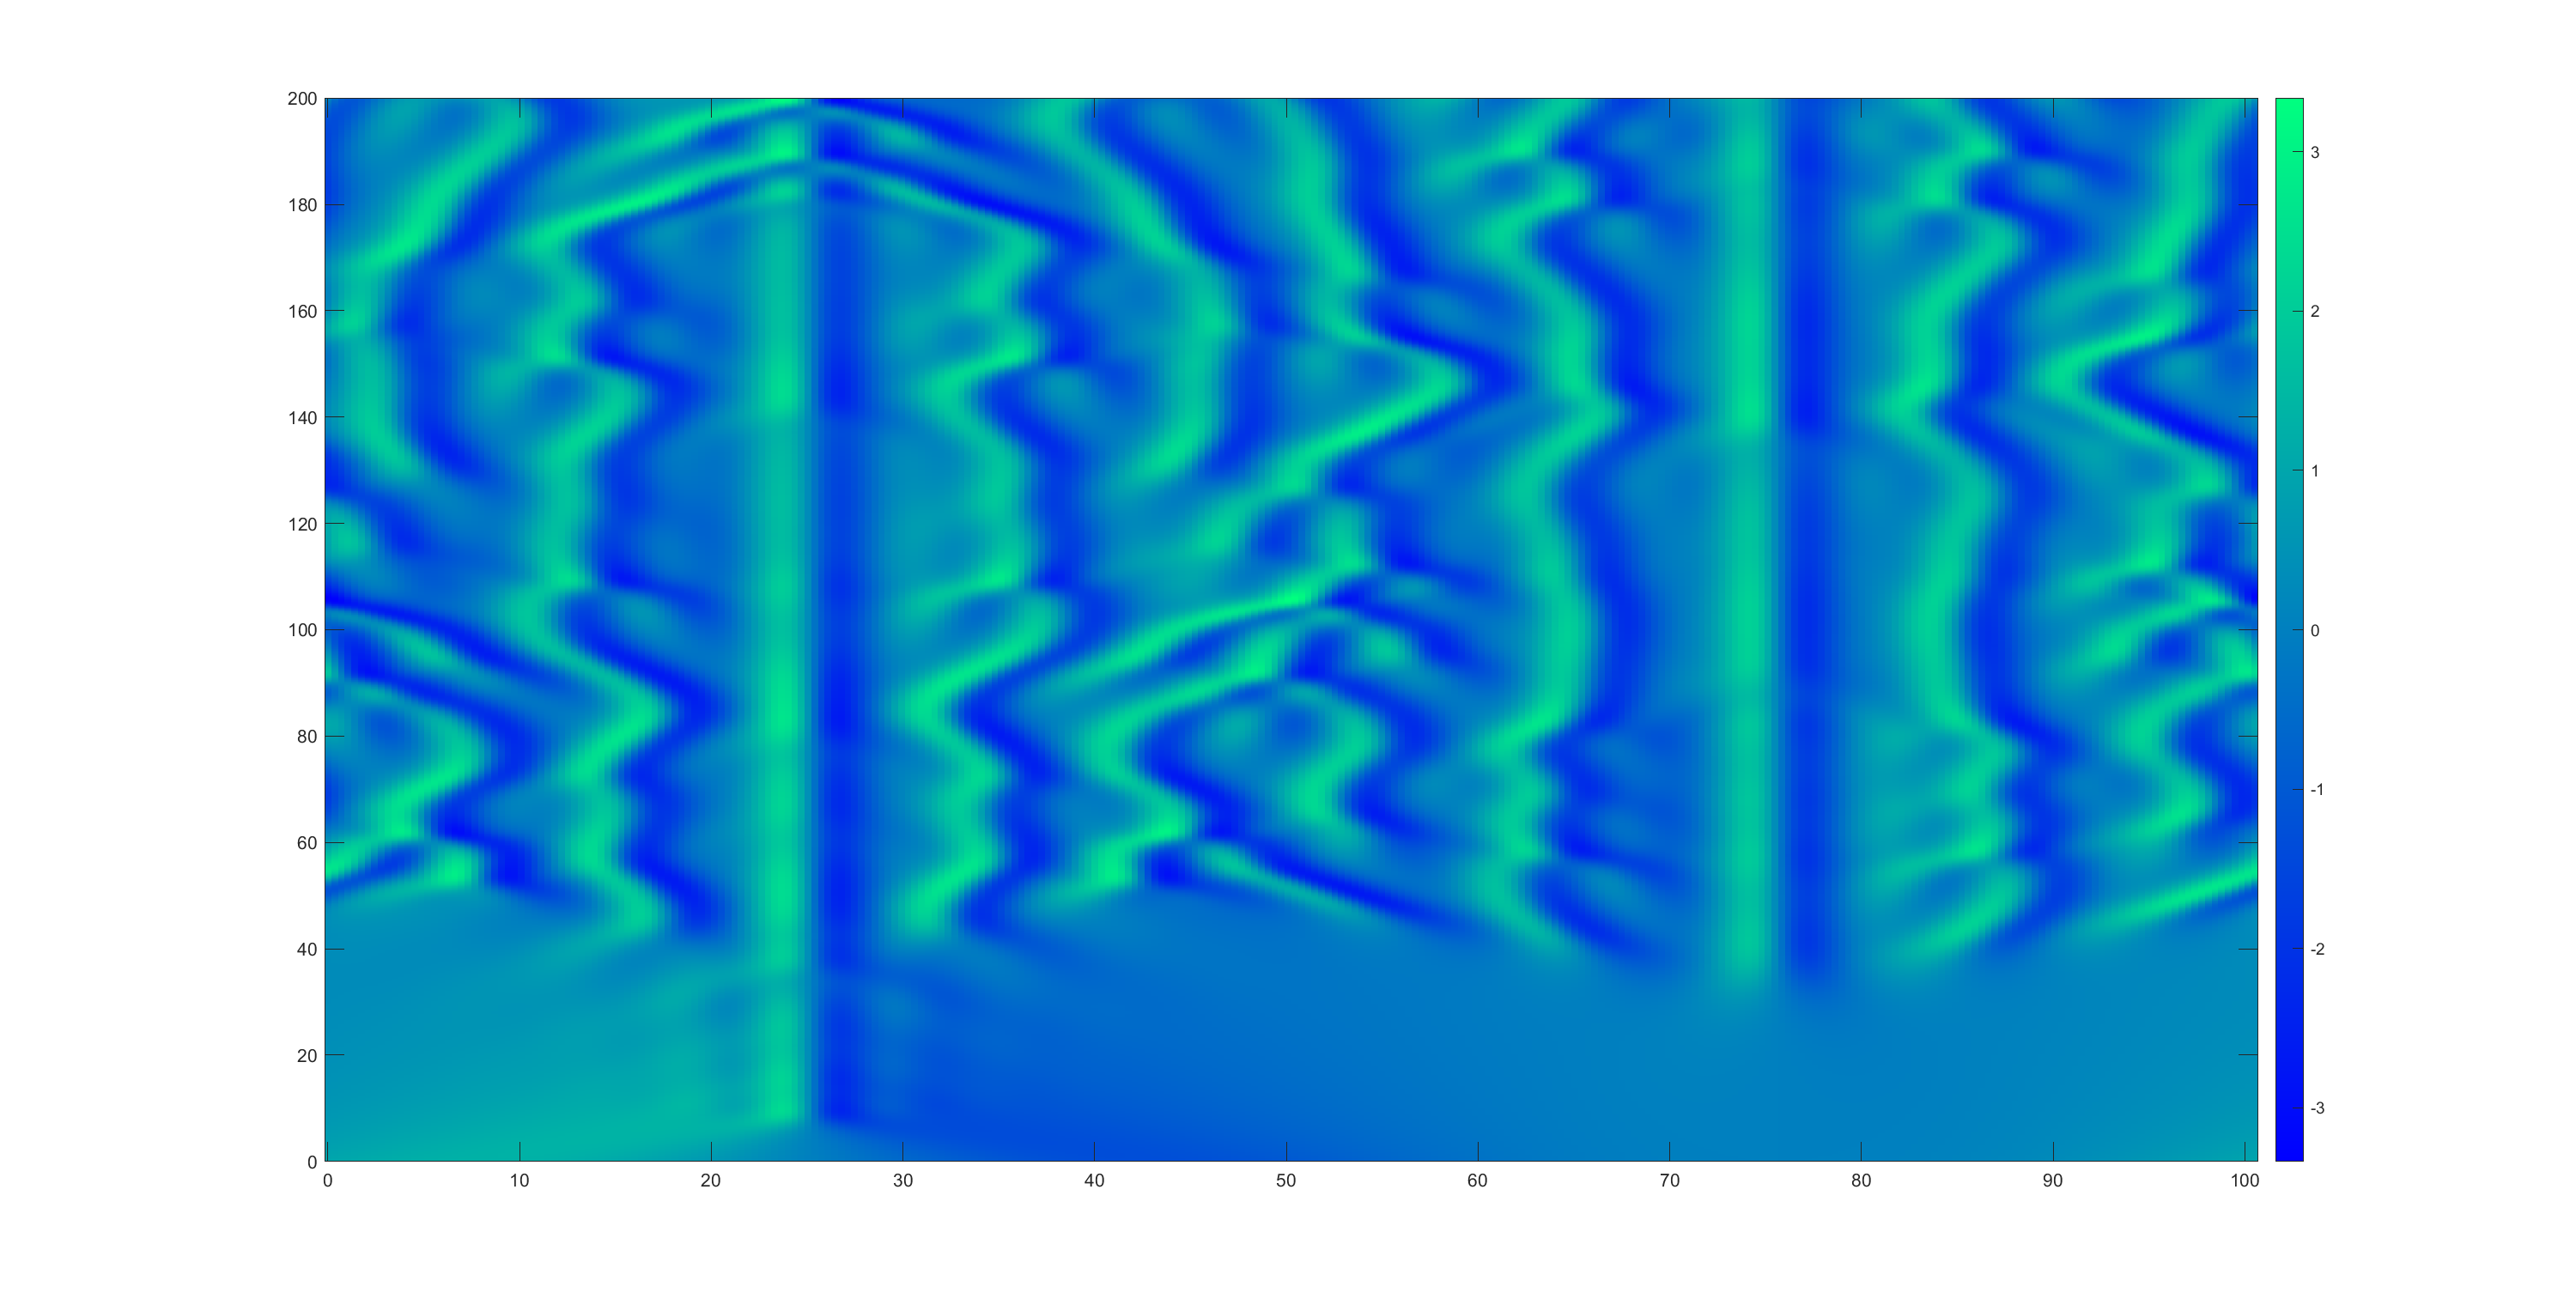
\includegraphics[scale=.3]{hw13 q4 plot}
\end{center}
The plot is very similar to the one in the linked article. The initial data does not vary significantly, but it splits into many high frequency waves, giving rise to a complex looking solution. On the other hand, characteristic lines appear, upon which solutions appear stationary, and moreover nearby solutions tend toward these lines. 
	
\end{document}